\section{Metodologia}
\label{sec:metodologia}

\subsection{Conjunto de dados e variáveis}
\label{subsec:dataset}

Utiliza-se o conjunto de dados \textit{Air Quality} do repositório UCI \textit{Machine Learning Repository}\cite{airqualityuci2008}, composto por medições horárias realizadas entre março de 2004 e abril de 2005 em um ambiente urbano ao nível da rua, caracterizado por elevada poluição atmosférica. O conjunto integra medições de referência de poluentes, respostas de uma matriz de sensores químicos de óxido metálico (MOx) e variáveis meteorológicas .

As variáveis foram organizadas em três grupos conforme sua natureza: (i) medições reais de referência (\textit{ground truth}), utilizadas como variáveis-alvo e de validação; (ii) respostas de sensores MOx, expressas em unidades arbitrárias (u.a.), que representam sinais elétricos internos dos sensores e não correspondem diretamente a concentrações físicas de poluentes; e (iii) variáveis ambientais, empregadas como preditores auxiliares. A Tabela~\ref{tab:stats-air-quality} apresenta estatísticas descritivas resumidas para cada variável, evidenciando diferenças de escala e de completude entre os grupos.

\begin{table}[htbp]
\centering
\caption{Estatísticas descritivas do conjunto de dados \textit{Air Quality}.}
\label{tab:stats-air-quality}
\begin{tabular}{l r r r r r}
\toprule
\textbf{Variável (unidade)} & \textbf{N} & \textbf{Vazios (\%)} & \textbf{Mín.} & \textbf{Média} & \textbf{Máx.} \\
\midrule
\multicolumn{6}{l}{\textbf{Medições reais}} \\
CO(GT) (mg\,m$^{-3}$)            & 7\,674 & 18,97 & 0,10 & 2,15 & 11,90 \\
C$_6$H$_6$(GT) ($\mu$g\,m$^{-3}$) & 8\,991 & 5,07  & 0,10 & 10,08 & 63,70 \\
NO$_x$(GT) (ppb)                 & 7\,718 & 18,51 & 2,00 & 246,90 & 1\,479,00 \\
NO$_2$(GT) ($\mu$g\,m$^{-3}$)    & 7\,715 & 18,54 & 2,00 & 113,09 & 340,00 \\
\textbf{NMHC(GT) ($\mu$g\,m$^{-3}$)} & \textbf{914} & \textbf{90,35} & 7,00 & 218,81 & 1\,189,00 \\
\midrule
\multicolumn{6}{l}{\textbf{Sensores MOx (resposta elétrica, u.a.)}} \\
PT08.S1(CO) (u.a.)   & 8\,991 & 5,07 & 647,00 & 1\,099,83 & 2\,040,00 \\
PT08.S2(NMHC) (u.a.) & 8\,991 & 5,07 & 383,00 & 939,15 & 2\,214,00 \\
PT08.S3(NOx) (u.a.)  & 8\,991 & 5,07 & 322,00 & 835,49 & 2\,683,00 \\
PT08.S4(NO$_2$) (u.a.) & 8\,991 & 5,07 & 551,00 & 1\,456,26 & 2\,775,00 \\
PT08.S5(O$_3$) (u.a.)  & 8\,991 & 5,07 & 221,00 & 1\,022,91 & 2\,523,00 \\
\midrule
\multicolumn{6}{l}{\textbf{Variáveis ambientais}} \\
T ($^\circ$C)        & 8\,991 & 5,07 & -1,90 & 18,32 & 44,60 \\
RH (\%)              & 8\,991 & 5,07 & 9,20 & 49,23 & 88,70 \\
AH (g\,m$^{-3}$)     & 8\,991 & 5,07 & 0,18 & 1,03 & 2,23 \\
\bottomrule
\end{tabular}
\end{table}

\subsection{Pré-processamento dos Dados}
\label{subsec:preprocessamento}

O pré-processamento teve como objetivo garantir consistência estatística e viabilizar a aplicação dos algoritmos de classificação. Os dados foram carregados respeitando o separador e a codificação decimal originais, e os valores ausentes identificados pelo código \texttt{-200} foram convertidos para valores nulos. Colunas sem informação relevante e registros incompletos foram removidos. A variável \texttt{NMHC(GT)} foi excluída devido à elevada proporção de valores ausentes (superior a 90\%), o que comprometeria a robustez das análises. Em seguida, o conjunto de dados foi particionado de forma estratificada em conjuntos de treino (70\%) e teste (30\%), preservando a distribuição das classes do índice de poluição.

As variáveis preditoras foram normalizadas por meio da padronização z-score, a fim de reduzir o efeito de diferentes escalas e unidades entre os atributos, garantindo que nenhum deles exerça influência desproporcional no modelo. Essa transformação contribui para maior estabilidade numérica e melhor desempenho dos algoritmos de classificação, sendo definida por:
\begin{equation}
z_i = \frac{x_i - \mu}{\sigma},
\end{equation}
em que $x_i$ representa o valor original da variável, $\mu$ sua média e $\sigma$ o desvio padrão calculado exclusivamente no conjunto de treino.

\subsection{Construção do Índice de Poluição Multivariado}
\label{subsec:indice_poluicao}

Com o objetivo de representar o nível global de poluição atmosférica de forma integrada, foi construído um índice multivariado a partir das medições reais de referência dos poluentes CO, C$_6$H$_6$, NO$_x$ e NO$_2$.

Inicialmente, cada poluente foi padronizado utilizando estatísticas robustas, baseadas na mediana e no intervalo interquartil (IQR), conforme:
\begin{equation}
x^{*}_{i} = \frac{x_i - \text{mediana}(x)}{\text{IQR}(x)},
\end{equation}
onde $\text{IQR}(x) = Q_3(x) - Q_1(x)$.

O índice de poluição multivariado foi então definido como:
\begin{equation}
\text{IP} = \frac{1}{P} \sum_{j=1}^{P} x^{*}_{j},
\end{equation}
em que $P$ representa o número de poluentes considerados.

A Figura~\ref{fig:eda_temporal_behavior} ilustra a evolução temporal mensal do índice de poluição multivariado ao longo do período analisado. Essa visualização permite verificar a coerência temporal do índice construído e sua capacidade de sintetizar a variabilidade conjunta dos poluentes considerados, sem introduzir instabilidades decorrentes do processo de agregação.

\begin{figure}[h]
\centering
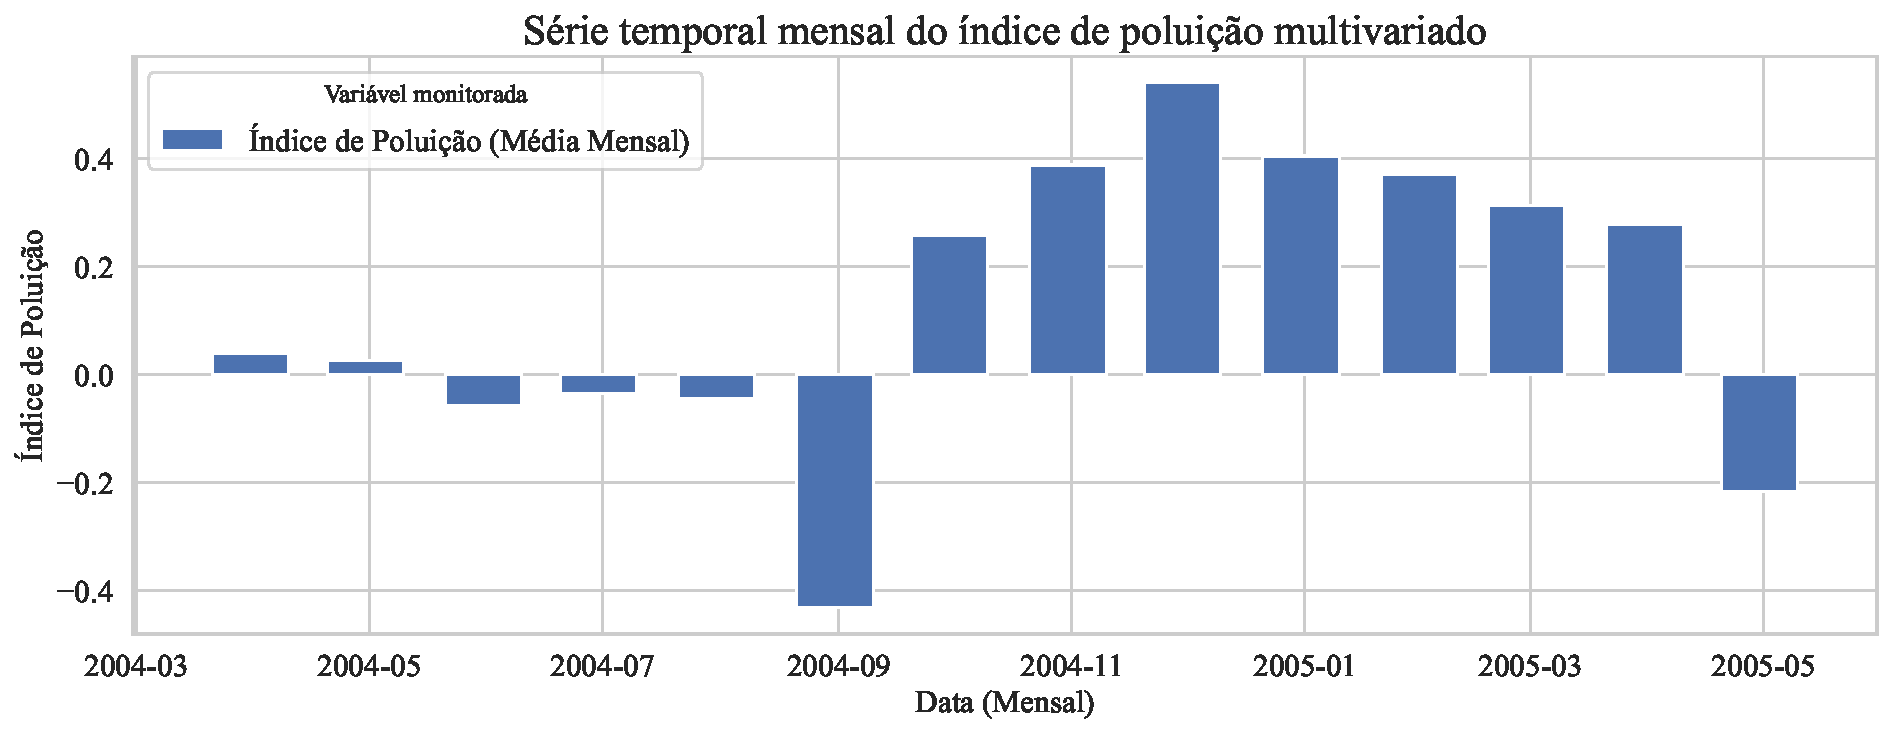
\includegraphics[width=\columnwidth]{figures/eda_temporal_behavior_monthly.pdf}
\caption{Série temporal mensal do índice composto de poluição.}
\label{fig:eda_temporal_behavior}
\end{figure}

Para a formulação do problema de classificação, o índice contínuo foi discretizado em classes ordinais por meio de quantis empíricos:
\begin{equation}
\text{Classe} =
\begin{cases}
C_1, & \text{IP} \leq q_{0.10} \\
C_2, & q_{0.10} < \text{IP} \leq q_{0.30} \\
C_3, & q_{0.30} < \text{IP} \leq q_{0.70} \\
C_4, & q_{0.70} < \text{IP} \leq q_{0.90} \\
C_5, & \text{IP} > q_{0.90}
\end{cases}
\end{equation}

A Tabela~\ref{tab:caracterizacao} apresenta a distribuição percentual das classes obtidas após a discretização do índice. A divisão balanceada decorre diretamente da definição dos quantis e estabelece um cenário experimental adequado para a avaliação comparativa de classificadores multiclasse.

\begin{table}[htb!]
  \centering
  \caption{Distribuição percentual das classes de poluição no conjunto de dados.}
  \label{tab:caracterizacao}
  \begin{tabular}{l c c c}
    \toprule
    Classe de poluição & Total (\%) & Treino (\%) & Teste (\%) \\
    \midrule
    Muito baixo & 10.01 & 10.00 & 10.03 \\
    Baixo       & 20.00 & 20.01 & 19.97 \\
    Moderado    & 39.99 & 40.00 & 39.99 \\
    Alto        & 20.00 & 19.99 & 20.02 \\
    Crítico     & 10.00 & 10.00 & 9.99 \\
    \bottomrule
  \end{tabular}
\end{table}

\subsection{Modelos de Classificação}
\label{subsec:modelos}
A modelagem teve como objetivo avaliar a capacidade de diferentes algoritmos de classificação em identificar corretamente os níveis de poluição a partir das variáveis preditoras. Todos os modelos foram implementados em \textit{Python} utilizando a biblioteca \textit{scikit-learn}, responsável pela padronização das variáveis, codificação do alvo, validação cruzada, treinamento e avaliação de desempenho, garantindo um protocolo experimental reprodutível e comparável entre as abordagens consideradas \cite{scikit-learn}.

\subsubsection{Modelos Lineares}
\label{subsubsec:modelos_lineares}

A Regressão Logística Multiclasse foi empregada como modelo discriminativo, estimando a probabilidade condicional das classes segundo a função \textit{softmax}:
\begin{equation}
P(y=k \mid \mathbf{x}) =
\frac{\exp(\mathbf{w}_{k}^{\top}\mathbf{x})}
{\sum_{j=1}^{K} \exp(\mathbf{w}_{j}^{\top}\mathbf{x})},
\end{equation}
onde $K$ representa o número de classes. O modelo foi ajustado utilizando o solver \textit{lbfgs}, adequado para problemas multiclasse, com limite máximo de 1000 iterações para assegurar convergência numérica.

Adicionalmente, utilizou-se a \textit{Linear Discriminant Analysis} (LDA), que assume distribuições gaussianas multivariadas com matriz de covariância compartilhada entre as classes e fronteiras de decisão lineares. O método projeta os dados em um subespaço que maximiza a separação entre as classes e minimiza a variância intra-classe, resultando em uma função discriminante linear. O modelo foi empregado em sua formulação clássica, sem regularização adicional, seguindo as hipóteses estatísticas padrão do método.

\subsubsection{Modelos Não Lineares}
\label{subsubsec:modelos_nao_lineares}

O \textit{k}-Nearest Neighbors (KNN) foi utilizado como método baseado em instâncias, classificando cada observação a partir da classe majoritária entre seus $k$ vizinhos mais próximos segundo a métrica euclidiana. O valor de $k$ foi selecionado por validação cruzada estratificada com cinco partições, considerando valores ímpares no intervalo $[1,49]$, e adotou-se ponderação dos vizinhos pelo inverso da distância.


Por fim, a \textit{Quadratic Discriminant Analysis} (QDA) foi empregada como extensão do LDA, permitindo matrizes de covariância distintas por classe e resultando em fronteiras de decisão quadráticas. Essa maior flexibilidade possibilita capturar relações mais complexas entre as variáveis preditoras quando comparada ao LDA. O modelo foi utilizado sem regularização adicional, explorando integralmente sua flexibilidade estatística.

\subsection{Avaliação de Desempenho}
\label{subsec:avaliacao}

O desempenho dos modelos foi avaliado exclusivamente no conjunto de teste. A métrica principal considerada foi a acurácia global, definida como:
\begin{equation}
\text{Acurácia} = \frac{1}{N} \sum_{i=1}^{N} \mathbb{I}(\hat{y}_i = y_i),
\end{equation}
em que $\hat{y}_i$ e $y_i$ representam, respectivamente, a classe prevista e a classe verdadeira da $i$-ésima observação.

A análise foi complementada por matrizes de confusão, apresentadas na Figura~\ref{fig:confusion_placeholder}, permitindo identificar padrões de erro e confusões sistemáticas entre classes adjacentes.

\begin{figure}[H]
\centering
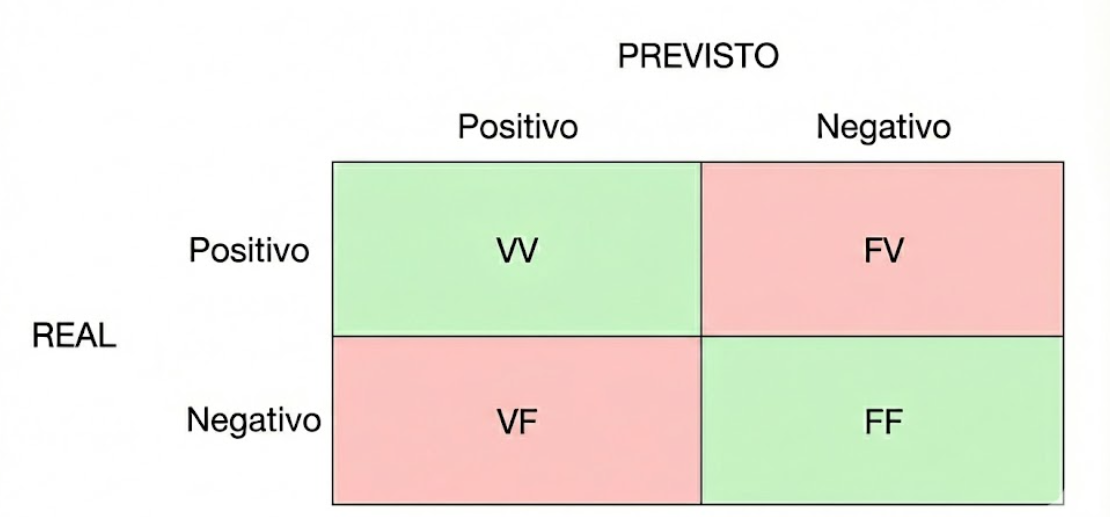
\includegraphics[width=0.4\textwidth]{figures/confusion_placeholder.png}
\caption{Exemplo de matriz de confusão para um dos modelos avaliados.}
\label{fig:confusion_placeholder}
\end{figure}
Adicionalmente, empregou-se o F1-score como métrica complementar, definido como a média harmônica entre precisão e revocação:
\begin{equation}
\text{F1}_c = \frac{2\,TP_c}{2\,TP_c + FP_c + FN_c},
\end{equation}
em que $TP_c$, $FP_c$ e $FN_c$ representam, respectivamente, os verdadeiros positivos, falsos positivos e falsos negativos da classe $c$.

Para avaliação global dos modelos em cenário multiclasse, adotou-se o F1-macro, definido como a média aritmética simples dos F1-scores das classes:
\begin{equation}
\text{F1}_{\text{macro}} = \frac{1}{K} \sum_{c=1}^{K} \text{F1}_c,
\end{equation}
atribuindo o mesmo peso a todos os níveis de poluição, independentemente de sua frequência.
